% !TeX root = ../../main.tex
\section{Architecture}\label{section:architecture}

The experiments presented in the next Chapter are implemented as part of the \gls{UBII} front end. The same applies to the smart device client, as illustrated in Figure~\ref{fig:architecture}. Both applications run in a web browser on the device and communicate with the \gls{UBII} server\footnote{Figure~\ref{fig:architecture} illustrates no direct connection between the smartphone/\gls{PC} and the \gls{UBII} server for the sake of simplicity. However, when running the software, one is actually established, since the \gls{UBII} front end runs on the client.}. In most scenarios, the smartphone is connected to the server via \gls{WLAN}.

\begin{figure}[H]
  \centering
  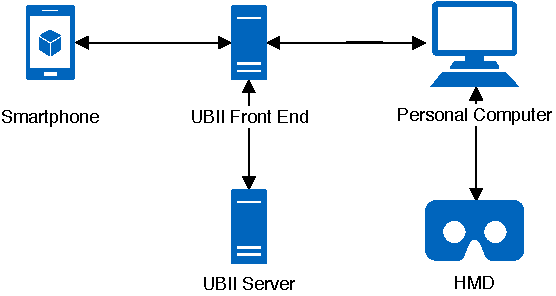
\includegraphics[width=10cm]{figures/implementation/architecture.pdf}
  \caption[The system architecture]{The architecture of the complete system. An arrow means that the connected applications communicate over the network with each other.}\label{fig:architecture}
\end{figure}

A \gls{PC} running the \gls{HMD} driver software and a web browser with the experiments running is used as a bridge between the \gls{HMD} and the \gls{UBII} front end. This setup may vary depending on the \gls{VR} headset. The Google Cardboard, for example, does not require any \gls{PC} in between.

